\documentclass[a4paper,12pt]{article}

%Packages
\usepackage{amssymb,amsmath}
\usepackage[T1]{fontenc}
\usepackage{lmodern}
\usepackage{array}
\usepackage{caption,txfonts,fontawesome,pifont}
\usepackage{graphicx}
\usepackage{booktabs}
\usepackage{tfrupee}
\usepackage{colortbl}
\usepackage[noblocks]{authblk}

\usepackage{setspace,tabularx}
\usepackage{array,multirow,ragged2e}
\usepackage[flushleft]{threeparttable}
\usepackage{float}
\restylefloat{table}
\usepackage{placeins}
\usepackage{subcaption}
%\usepackage{subfigure}
%colours


%Definitions
\providecommand{\keywords}[1]
{
	\small	
	\textbf{\textit{Keywords:}} #1
}



%opening
\title{Assymetric Impact of Oil Price on Food Prices in India: Evidence from NARDL Approach}
\author{%
Mohammed Shameem P \thanks{Corresponding Author(email:mohammedshameemp@gmail.com) School of Economics, University of Hyderabad} ,
Nithin M \thanks{Department of HSS, Indian Institute of Technology- Kharagpur},
xx \thanks{xx}
}

\date{}

\begin{document}

\maketitle

\begin{abstract}
Rising food prices have always been a cause of worry in India. Such episodes of rising food prices have always created large hue and cry among the masses which has stimulated extensive political and academic discussions on causes and its implications. With the need to design policies to contain food inflation, numerous studies have examined the determinants of food prices. Oil prices have been traditionally thought of as one of the key determinants of food prices in India. Though the relationship between food and oil prices has been well established in the literature wih a symmetric relationships, this study employs the NARDL approach to examine the potential asymmetries in oil price pass-through to food prices. The study finds the presence of significant asymmetry in oil price pass-through to food prices in the long run. The study also finds that this asymmetry, however, is not significant in the short-run. The study hs important policy implications regarding oil price pass-through and market power. 
\end{abstract}

\keywords{Food Inflation, Oil Price pass-through, Asymmetric cointegration, NARDL}	


\section{Introduction}
\onehalfspacing
Inflation and inflation controlling is a matter of public concern in countries across the globe as increased prices deny access for consumption to the masses. Crude oil and food are two inevitable components in economic development and the basic life of people. The unprecedented fluctuations in the prices of these will have serious implications on energy and food security for any country. For common people, their income fails to increase with changes in prices always, which limits their consumption. On a macro level, fluctuations in the prices of oil and food will have repercussions on the employment rate, interest rate, inflation rate, and economic growth of a country, thus in both ways, the dynamics of these prices are a concern for policymakers. Determinants of Inflation and its facets shows transition in India, especially after the global financial crisis. (Mohanty and John, 2015). The heavy reliance of the Indian economy on international markets for its oil requirements makes domestic prices sensitive to changes in international oil prices (Sabyasachi and Bhattacharya, 2011). The administrative oil price regime in India played the role of shock absorber for a long time. The objectives of such a system were to safeguard the public from the direct impact of oil price hikes in the international markets. But this mechanism could only ensure postponement of inflationary pressures which subsequently realized (Bhattacharya and Bhattacharyya, 2001). Later this system was lifted and thus price changes in the international market started reflecting in domestic prices. The impact of increased oil prices is not homogenous across the countries. The effects will be deeper in developing countries than in developed countries. The inadequate oil-conservation techniques and oil dependence of the production process in these countries are considered as the reasons for this imbalance (Bhattacharya and Bhattacharyya, 2001; Varghese, 2016).

The increase in crude oil prices will influence the economy in multiple ways. An increase in energy bills of households, industry, and government as they are direct consumers of the oil may end up in a slowdown of consumption expenditures in the economy. This will work as a rise in the unit cost of production for industries and agriculture Tang et.al (2009). These changes will ultimately visible on productivity, real wages and employment, selling prices, core inflation, profits, and investment in the economy. Empirical estimation using econometric models has revealed that the impact of crude oil prices on economic variables are not homogeneous in nature (Bhattacharya and Batra, 2009). Moreover, the repercussions of price hikes on economies depends on the level of economic development and position in the world trade.  In developing countries food is a major component in the consumption basket, which makes food prices a major driver of general consumer prices in the country and affects the poor sections of society deeply
(Jongwanich and Park, 2011; Bhanumurthy et al., 2012). Here the increase in oil price will couple with food prices and the joint effect on the economy will be greater (Alghalith, 2010). As matter of fact, on a global level, the majority of poor countries in the world are net food importers. Which makes them more affected by higher food prices (Ng and Aksoy, 2008). And thus, for oil-importing poor and developing countries higher oil and fuel prices endanger their energy security and threaten their food security (Hesaryet.al, 2019).

The heterogeneity in the impact of oil prices on world economies motivated wide research on the fuel-food co-movement. The history of researches on the co-movement shows that the context of each study was different for different countries and time. The theoretical and empirical studies primarily brought explanations to the link between energy and agricultural commodities and then draws further conclusions on their behavior. In the case of India, the most relevant conclusion on the tradeoff between oil and food prices are based on the Cost-push hypothesis. Even though in the literature, empirical evidence for other rationales viz based on higher demand for biofuels, effects of general inflation, and recent financialization are also prominent, but their relative significance is limited in the Indian context. According to this, the conventional transmission mechanism, oil price significantly affects the production cost of agricultural outputs and thus food prices (Hanson et al., 1993; Baffes, 2007; Esmaeili and Shokoohi, 2011; Hesary et.al, 2019) which will pass to the final prices. Oil and oil derivatives are used in primary and secondary stages of agricultural production in various factors. Considering the supply side, changes in oil prices will have its impact on cost of these factors.

Generally, inflation in India had stayed at an average of 6.7 percentage for a period from 1950 to 2013 which shows that WPI inflation is modest in the country (Mohanty and John, 2015). Different factors triggered the occurrences of high food inflation in India over the years. Recent trends in inflation are mainly explained in the literature focusing on demand-side factors (Nair and Eapen, 2011; Basu, 2011; Chand, 2010; Kumar, 2010). The strong inflationary pressure in the country especially since 2007 is well associated with a large share of food and fuel products in total consumption. The role of cost push supply shock in food prices, along with oil prices are considered as critical in inflation in India (Bhanumurthy et al., 2012; Holtemoller and Mallick, 2016; Nair and Eapen, 2012).

Considering Oil prices as one of the key determinants of food inflation in India, there is a need for a meticulous assessment of the tradeoff between oil and food prices. The co-movement of oil prices and food inflation (and general inflation) has been assessed and addressed extensively for many economies in the world. In the Indian context, the relationship between food and oil prices has been well established with symmetric relationships, in the literature. This paper is an attempt to address the potential asymmetries in their behavior. A co-integration analysis of oil prices and food prices in India for the period 2012-2016 (monthly data) is the purpose of this paper. Using the newly introduced Wholesale Price Index-based food index with the base year 2011-12 series along with WTI (Western Texas Intermediate) crude oil price a non-linear autoregressive distributed lag (NARDL) model is proposed. Even though food and food-related items hold a significant share in both of the major indices used in measuring inflation in India, by Using Wholesale Price Index (WPI) monthly data, the study enables to analyze food inflation from the supply side as WPI is considered as a producer’s index.

The structure of the paper is as follows: Section briefs the existing literature on the co-movement between oil prices and inflation. A description of the Data and methodology to be used in the analysis is discussed in Section 3. The empirical result and discussion are part of Section 4. The conclusion along with relevant policy implications are explained in final section

\section{Review of literature}
The relationship between energy and food prices has been analyzed extensively in the literature. 
There is a general conscience extracted from several studies regarding the influence of oil price movements on economic variables, which in fact depends on multiple factors including structure of the particular economy, energy intensity of sectors etc. (Tang et.al .2009). Hamilton's (1983)’s seminal work was the early attempt in assessing the influence of oil price on the performance of the economy. Hamilton’s study pointed out the oil-price dynamics as a significant factor in recessions in U.S economy after World War II. This study was followed by a series of studies to explore this relationship between oil-price shocks and the various aspects of the aggregate economic performance of various nations. This was aggravated by oil politics and its effect on the world’s major economies in the second half twentieth century. Different transmission channels of Oil prices pass through to macro-economic variables were identified. The classical supply-side effects cost of basic inputs for production through an increase in oil prices increase (Barro, 1984). This is the most widely accepted explanation for the question on relationship of oil and agricultural product prices.

The cost-push inflation effect of oil price increase was discussed by many studies. A positive relationship between energy products prices and food prices in long-run were established in a world computable general equilibrium model by Gohin and Chantret (2010). Jongwanich and Park (2011) the empirical assessment of the pass-through of international food and oil prices to domestic consumer prices in nine Asian countries. The study holds structural factors such as the economic transformation in China and India, as the major driver of increased global food and oil prices during 2007 and 2008. Esmaeili and Shokoohi (2011) evaluated the impact of crude oil prices on world food price changes using principal component analysis (PCA). The study explained the indirect effect of crude oil prices on food prices by the pass-through of influence of oil price index on the food production index and thus on the macroeconomic index.  But no direct long-run co-integration between time series prices of fuels and agricultural commodities was found by Zhang et al. (2010).

Nazlioglu and Soytas (2012) investigated the evidence for the one-way dynamics of agricultural commodity prices and world oil prices. The study was on 24 selected commodities on their monthly prices from January 1980 to February 2010. The empirical results of panel cointegration and Granger causality methods confirmed this strong relationship. The structural VAR model of Wang et.al (2014) shows that during the post-crisis period (2006-2008) the influence of oil supply shock on agricultural commodity prices has increased drastically. In a panel framework, the analysis by Rezitis (2015) found a two-way Granger causality between crude oil prices and agricultural product prices and fertilizer prices for the period from June 1983 to June 2013. The wavelet coherence analysis of Pal and Mitra (2017) found a significant trade off between world food prices and oil prices.

The influence of changes in prices of oil products on the Chinese economy and its price transmission mechanism was evaluated by Tang et.al (2009) using the structural vector autoregressive model, the empirical results confirmed the positive relationship between oil prices and inflation rate and interest rate in the economy. The significant influence of both expected and unexpected oil price shocks on the Chinese commodity market was showed in the study of Zhang et al. (2018).
Using a structural vector autoregressive (SVAR) model Ahmed and Wadud (2011) explain that the positive oil shocks hurt the level of inflations in Malaysia. Alghalith (2010) indicated a positive relationship between food price and oil price for Trinidad and Tobago. The study explains potency of oil price volatility on movement of food price in the economy.

Globally the increase in the oil prices resulted in considering corn-based ethanol and soybean-based bio-diesel as alternatives for traditional crude oil. This shift resulted in a new spectrum in the importance of these grains and its prices. Chen et.al (2010) presented evidence for influence of crude oi prices on world prices of grains like corn and soybean, through a derived demand. The findings of the bivariate VAR-Generalized Autoregressive Conditional Heteroskedasticity (VAR-GARCH) model from Al-Maadid et al. (2017) explains both mean and volatility spillover in the ethanol and food prices trade off.

The empirical results of the study by Haixia and Shiping (2013) on prices of oil, corn and ethanol in Chinese economy also shows a one-way spillover effect . 
The EGARCH and BEKK-MVGARCH models estimated, for the period September 2003 to August 2012, reveal this one-way spillover effect a of oil prices on corn and ethanol prices. As explained earlier this relationship based on derived demand is not significantly proved in the case of India. Some studies contradict this notion even for advanced economies like the US. The study of Baumeister and Kilian (2014) on US retail food price and oil prices were completely contradicting the general notion regarding the co-movement of these variables along with the conscience on cost-push food inflation by oil prices hikes. The study explains that there is no evidence for any close influence of oil prices on US retail food prices before or after the 2006 US biofuel policies. Gardebroek and Hernandez (2013) also concluded the absence of any volatility spillover effect of oil market on the corn market in the US using used the multivariate GARCH model.


The majority of the literature on interrelation between energy GDP and later oil prices and GDP and other macro variables including inflation was primarily aimed at finding the presence of long-term relationships between these variables. The basic premises of these studies were based on the usual linear cointegration models. The episodes of oil price falls in the 1980s raised questions compatibility of these models based on linear relationships as the macroeconomic variables followed a contradictory path. This motivated researchers to address the asymmetries in these relationships. Few studies explained the dynamic relationships between these variables in an asymmetric framework. Mork, 1989; Mory, 1993; Brown, and Yücel, 2002. The nonlinear versions of autoregressive distributed lag (ARDL), Granger causality, and vector error correction models (VECM) models are mainly used by major studies. In the estimated results of the study by Lardica and Mignon (2008) the standard cointegration was not significant between oil prices and GDP, whereas the asymmetric cointegration between variables were found.

Nonlinear relationship between prices of ethanol and oil were found by Balcombe and Rapsomanikis (2008) for the country Brazil using a generalized bivariate error correction model.
Same way, a nonlinear relationship between energy and food prices was identified by Serra et al., (2011) for the U.S ethanol industry.

In the case of china, Du et.al (2010) established the non-linear impact of world oil price on economic growth and inflation using the multivariate vector autoregression (VAR) model.
Nazlioglu (2011) estimated the relationship of world oil prices on prices of corn, soybeans, and wheat using both linear and nonlinear Granger causality tests. When the neutrality hypothesis was established from linear causality tests, a unidirectional nonlinear causality was evident from the prices of oil to prices of corn and soybeans.
A nonlinear autoregressive distributed lags (NARDL) model was used to analyze the oil- food price link in Malaysia (Ibrahim, 2015). It was found that oil price decline was not having a significant impact on food prices while prices hikes in oil markets had significant repercussions in food market.

Employing both nonlinear ARDL models and nonlinear Granger causality tests Rafiq and Bloch (2016) presence of non-linearity in the influence of oil prices on prices of twenty-five products prices for the period of 1990 to 2011.
Pal and Mitra (2017) explained the non-linearity in the effect of diesel prices on prices of soybean in US. The estimated results show that diesel prices exert higher pressure on soybean prices in higher quantiles. 

Eissa and Refai (2019) employed both the Nonlinear Autoregressive Distributed Lag (ARDL) Model of Shin et al. (2014) and the linear ARDL Model of Pesaran et al. (2001) to study long run relationship of price of agricultural commodities and oil. The co-movement was evident for the period 1990 - 2018 only in results of NARDL model. 

There are few notable studies about the co movement of oil prices, inflation, and output in India.  Studies specific on the impact of oil prices on the dynamics of food prices in the Indian market are limited.  These studies have shown the presence of both linear and nonlinear relationships between these variables. A bidirectional causality between oil and non-oil inflation was found by Bhattacharya and Bhattacharyya (2001) using a multivariate VAR model based on monthly data from April 1994 to December 2000. The study shows that a positive oil shock results an increase in inflation and a decrease in output. This stagflation induced by oil price shock in the Indian economy was examined by Bhattacharya and Kar (2005) and further stated that the deceleration of growth as the effect of oil price shocks were presented in long run.
Industrial growth and effects of oil price shocks were examined by Kumar (2005) for the period 1975-2004. The results Multivariate VAR model specified the negative effect of oil price shocks on the growth of industrial production.

A sector wise analysis of Kar and Bhattacharya (2011) stated that the fluctuations in oil prices affect the agricultural and tertiary sectors more and the impact of oil price shocks on these sectors were long-run in nature. According to Kaushik and Indranil (2011), the role of administrated prices and the lag in their price adjustments has produced bigger shocks in the economy.
Different macroeconomic indicators of Indian economy like output growth, inflation etc. were studied on the basis of the effects of international oil price shocks on them by Bhanumurthy et al. (2012).
. The study found differential impact on these variables and further examined these impacts along with different levels of pass-through. The study discussed two scenarios; partial pass through and full pass through of international oil price shocks. In the former case, a 10 percent rise can bring 0.3 percent rise in inflation whereas and if it is full pass-through then it would result in a 0.6 percent increase in inflation 

In the Commodity-wise study about the Causal Factors Food Price Inflation in India, Nair and Eapen (2012) found that in the period from March 2008 to November 2008 and January 2010 to July 2010, the surge in international oil prices were transmitted to the Wholesale Price Index (WPI) inflation rate of mineral oils .the study also concluded that food prices in Indian market is affected by higher oil prices.

Alom et al. (2013) examined the dynamics of world oil prices and food prices on a few Asian and Pacific economies. The basic premise of the study was that the characteristics of a particular economy will be the deciding factor in the magnitude of the effects of external price shocks. The structural vector autoregression (SVAR) models concluded that in the Indian economy, the impact of world oil price shocks was comparatively lesser than the impact of food price shocks. 
The multivariate vector autoregression (VAR) model of Bhat (2014) confirmed the asymmetric nature of the influence of oil price shocks on the Indian economy. The study explains exogeneous nature of macro-economic movement in India to oil prices changes for the period April 1992 to August 2013.
Mohanty and John (2015) identified crude oil prices as one among the major determining factors of inflation level in Indian market. The quarterly data based Structural vector autoregression (SVAR) model indicated that the in the period 2009–2010 and most of 2010–2011, changes in world oil prices determined inflation level in India with an impact of above 20 percent and later after 2011-2013 below 20 percent. 

In the transmission channel of crude oil prices and oil product prices, asymmetry was found by Pal and Mitra (2016). The Multiple threshold nonlinear autoregressive distributed lag (MTNARDL) model decomposed the price changes of crude oil holding multiple thresholds and confirms that the asymmetric price transmission., oil product prices move together with crude oil prices when it goes up, but fail to follow when there is a significant fall in crude prices.

The Structural Vector Autoregressive (SVAR) model analysis of Ahmed, K (2019) on how oil price shocks affects inflation rates of five SAARC countries including India confirms the variables are cointegration and long-run relationships between the variables.

Empirical results of the Structural vector autoregression (SVAR) model by Javed et. al (2018) also concluded asymmetric impact oil price shocks on output in the economy where price inflexibility or inflation rigidity was evident even in the long run (April 1994 to May 2016).   

In a study examining linkages between of eight Asian economies including India, confirms that energy price (oil price) has a significant impact on food prices. 
The study by Hesary et.al (2019) employed a Panel-VAR model for the period 2000–2016 on the relationship of energy price and prices of food products.
The study confirmed the significance of oil prices in determining food prices in India.  The impulse response functions showed that any shocks from oil prices had positive changes on agricultural food prices.

\section{Data and Methodology}
The study employes monthly data from 2012 April to 2017 March. The food price is measured by the newly introduced WPI based Food Index with the base year 2011-12. Oil price used for the study is measured using West Texas Intermediate crude oil price in both US dollar (USD) and Indian rupees (INR). The price of oil in Indian rupees is calculated by multiplying the US dollar price by the exchange rate in the corresponding month. 
\begin{align*}
	OP_{rs}=OP_{dol} \times er
\end{align*}
Where $OP_{rs}$ refers to the oil price in Indian rupees, $ OP_{dol} $ is the price of oil in US dollar and er refers to the exchange rate of vis-à-vis the US dollar. All the data is sourced from RBI database on Indian economy and Federal Reserve Bank of St. Louis (FRED). 

Oil price and food price have a strong impact on other macroeconomic variables. Both these variables exhibit strong trend which makes them non-stationary.  The standard methods of dealing with series that are non-stationary and exhibit relationship among them are the method of co-integration, error-correction and Granger causality. While these techniques enable in analysing the long-run and short-run relationships among the variables, they presume symmetrical relationship between them. Presence of asymmetry makes these models incapable of capturing potential asymmetric relationship that may exist between these variables.  Following Shin et al. (2011) we employ Non-Linear Autoregressive Distributed Lag Model (NARDL) approach to co-integration to capture this asymmetric relationship between oil price and food price in India. NARDL approach is an asymmetric extension to the more popular ARDL model of Pesaran and Shin (1998) and Pesaran et al. (2001).

Following Shin et al. (2011), we specify the long run equation of food price as below
\begin{equation}
	fp_t=\alpha_0+\alpha_1OP_t^++\alpha_2OP_t^-+\epsilon_t
\end{equation}
Where $ fp_t $ refers to the food price at time t and  $ OP_t $ refers to the oil price at time t and $ \alpha= [\alpha_0,\alpha_1,\alpha_2] $ is the vector of long-run parameters to be estimated. Also, $  OP_t^+ $ and $OP_t^- $ are partial sums of positive and negative changes to oil price. 
We decompose partial sums as follows
\begin{subequations}
	\begin{align}
		OP_t^+ = \sum_{i=1}^{t}\Delta OP_t^+ =\sum_{i=1}^{t}max(\Delta OP_t^+) \\
		OP_t^- = \sum_{i=1}^{t}\Delta OP_t^- =\sum_{i=1}^{t}max(\Delta OP_t^-)
	\end{align}
\end{subequations}
$\alpha_1$ captures the long-run relationship between food and oil price increase at time t while $\alpha_2$ indicates the long-run relationship between food and oil price reduction. Both these coefficients are expected to be positive. Based on theory and existing literature, we also expect that oil price increase will result in an increase in food prices at a greater magnitude than the corresponding reduction in food prices with reduction of oil prices in the long-run implying $\alpha_1$> $\alpha_2$.  This results in the long-run asymmetry of oil price pass through to food prices. 

As illustrated by Shin et al. (2011), the concept of partial asymmetry can be incorporated into the popular ARDL framework of Pesaran and Shin (1998) and Pesaran et al. (2001) to formulate an asymmetric error correction model as:
\begin{equation}\label{eq3}
	\Delta fp_t=\alpha+\sum_{i=1}^{n}\beta_ifp_{t-i}+\delta_1OP_{t-1}^++\delta_2OP_{t-1}^-+\sum_{j=1}^{p}\gamma_j \Delta fp_{t-j}+\sum_{k=1}^{q}\left(\theta_k^+ \Delta OP_{t-1}^++\theta_k^+ \Delta OP_{t-1}^-\right)
\end{equation}
	Where n,p and q represent lag orders and $ \alpha_i = - \frac{\delta_i}{1-\sum_{j=1}^{n}\beta_j}$ measures the long-run impacts of oil price increase and decrease on the food price. Similarly,  $\sum_{i=0}^{s}\theta_i^+$ and $\sum_{i=0}^{s}\theta_i^-$  measures the short-run influence of oil price increase and oil price decrease on food prices respectively.  
	
	There are few caveats to adhere to for empirical implementation of NARDL models. First is to ensure that none of the variables are integrated of order two. While NARDL models can be used for both I(0) and I(1) variables, it cannot be used for I(2) variables. The study uses popular ADF and PP tests for determining the order of integration of the variables. After ensuring that the variables are of order I(0) or I(1) we proceed to estimate \eqref{eq3} using standard OLS technique. Following Katrakilidis and Trachanas (2012), a general to specific approach is adopted to arrive at the optimal lag specification of NARDL model. Following Pesaran et al. (2001) and Shin et al. (2011), we employ bounds testing to test for cointegration among the variables which involves  Wald F test of the null hypothesis of no co-integration among the variables. With the evidence for co-integration among the variables, we derive the asymmetric long-run coefficients and make inferences. We also derive the asymmetric dynamic multipliers of 1\% change in $ OP_i^+ $  and $ OP_i^- $respectively as: 
	\begin{equation}
			mh^+= \sum_{j=0}^{p}\frac{\partial y_{t+j}}{\partial OP_{t-1^+}}\; \; \; \; mh^-= \sum_{j=0}^{p}\frac{\partial y_{t+j}}{\partial OP_{t-1}^-}
	\end{equation}
as h $\rightarrow \infty$, $ m_h^+ \rightarrow \alpha_1 $ and $ m_h^- \rightarrow \alpha_2 $.

\section{Results and Discussion}

Before we undertake analysis, we plot these variables to understand how they behave over time. It will also help in providing some idea about the potential relationship between these variables. The figures are given below
\begin{figure}
\centering
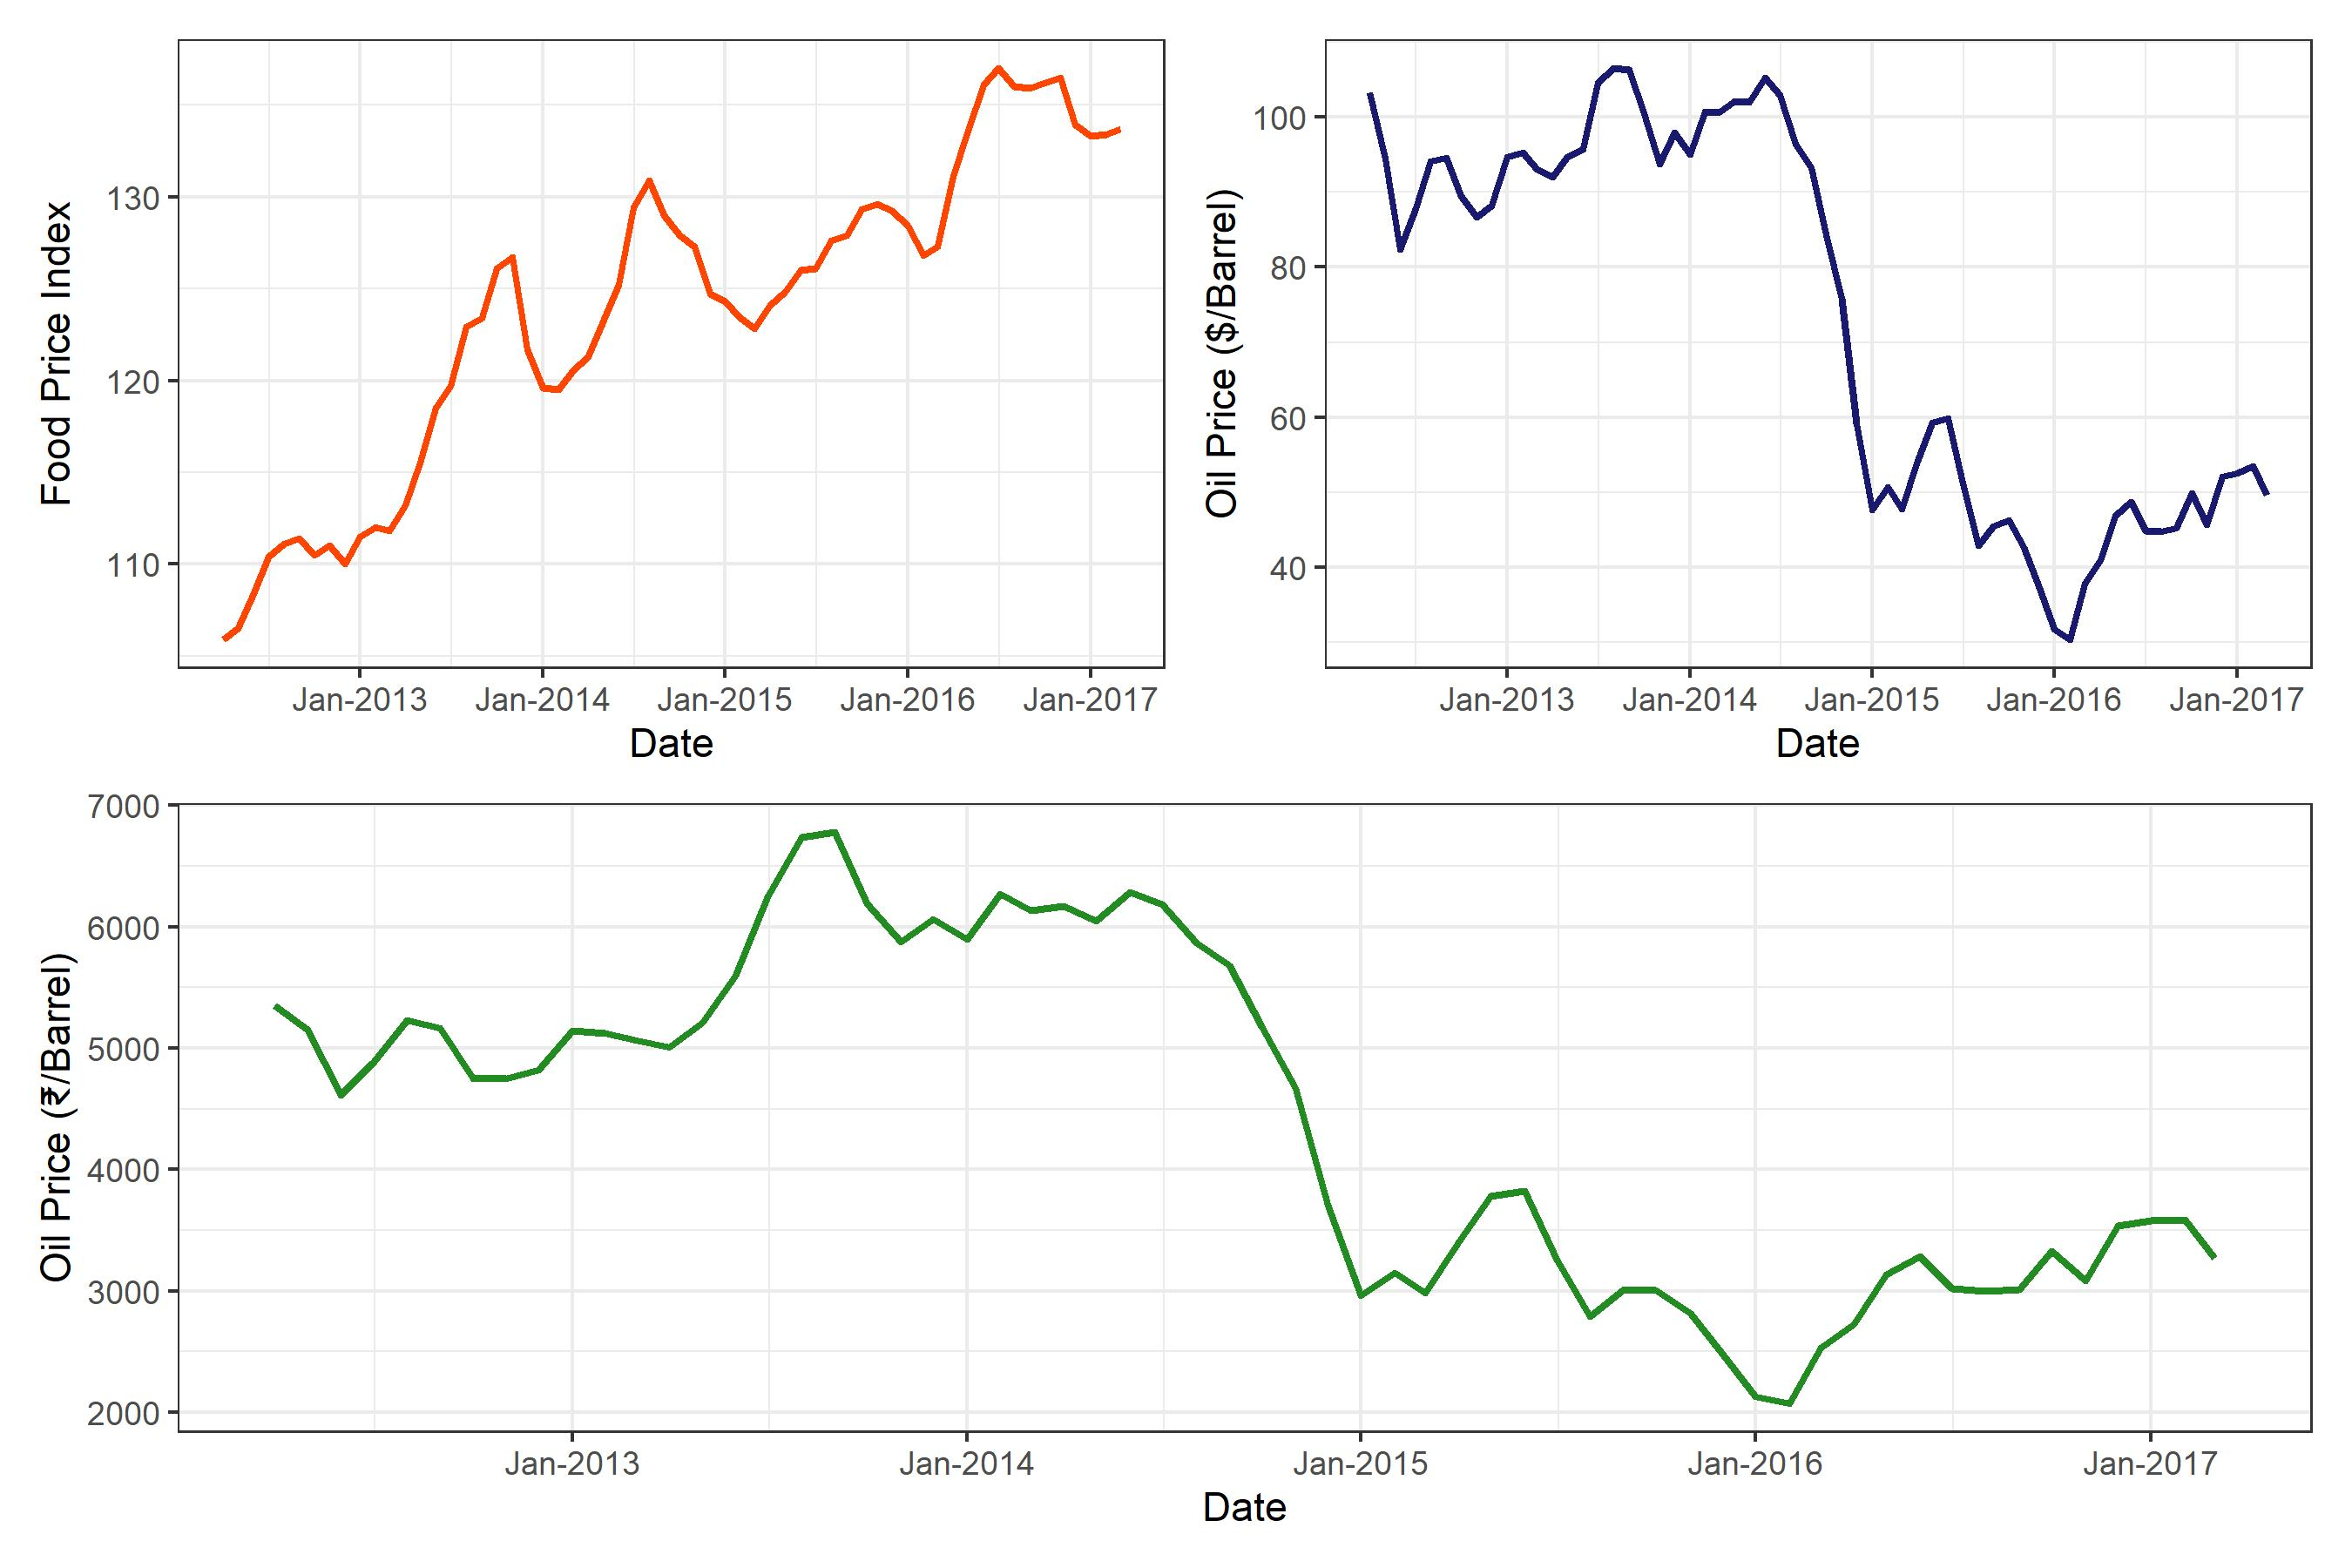
\includegraphics[scale=0.5]{new_trend.jpg}
\end{figure}

From the figures, it can be inferred that variables exhibit strong trend and are non-stationary. It is also observed that food price and oil price tend to move together in case of a price rise or a price fall. Since non-stationary time series are subject to the problem of spurious regression, we proceed to check the order of integration of these variables employing the popular ADF(Augmented Dickey-Fuller) and PP( Philips Perron) tests. This is a pre-requisite given the requirements of the bounds testing approach that none of the variables are integrated of order two. The results of these tests are given in the table below

\renewcommand{\arraystretch}{2.5}
\begin{table}[h]
	\large
	\begin{threeparttable}
			\resizebox{1.1\textwidth}{!}{%
		\begin{tabular}{ccccccccc}
			\hline
			\multirow{3}{*}{Variables} & \multicolumn{4}{c}{Level}                        & \multicolumn{4}{c}{First Difference}             \\ \cline{2-9} 
			& \multicolumn{2}{c}{ADF} & \multicolumn{2}{c}{PP} & \multicolumn{2}{c}{ADF} & \multicolumn{2}{c}{PP} \\
			& Intercept & Trend and Intercept & Intercept & Trend and Intercept & Intercept & Trend and Intercept & Intercept & Trend and Intercept \\ \cline{2-9} 
		Food price $\left(fp\right)$	& -1.806     & -3.435*    & -1.744     & -2.52     & -4.667***  & -4.694***  & -4.707***  & -4.739*** \\
		Oil Price in Dollar $\left(OP_{dol}\right)$	& -2.736*    & -2.8333    & -2.392     & -2.449    & -7.572***  & -7.606***  & -7.524***  & -7.606*** \\
		Oil Price in Rupees $\left(OP_{rs}\right)$	& -2.689*    & -2.558     & -2.299     & -2.166    & -7.778***  & -7.804***  & -7.857***  & -7.884*** \\ \hline
		\end{tabular}%
	}
\end{threeparttable}
\begin{tablenotes}
	\tiny
	\item *,** and*** denotes significance ate 10\%, 5\% and 1\% respectively. AIC (Akaike Information Criteria) was used to choose the optimum lag structure.
\end{tablenotes}
\caption{Unit-root tests}
\end{table}

The results of both the test indicate that none of the variables are integrated of the order two thus fulfilling the requirements for bounds testing procedure. Accordingly, we proceed to estimate equation \eqref{eq3}.The lag structure is chosen based on AIC criteria and is well in accordance with theory.

% Please add the following required packages to your document preamble:
% \usepackage{graphicx}
\renewcommand{\arraystretch}{1.3}
\begin{table}[h]
	\resizebox{\textwidth}{!}{%
		\begin{tabular}{cccc}
			\hline
			Model   & Dependent Variable & Independent Variables & Lag Selection \\ \hline
			Model 1 &     $fp$               &    $OP_{dol}^+,OP_{dol}^-$                   &  (2,2,2)             \\
			Model 2 &   $ln\_fp$                 &  $ln\_OP_{dol}^+,ln\_OP_{dol}^-$                     &  (2,2,2)              \\
			Model 3 &     $fp$               &      $OP_{rs}^+,OP_{rs}^-$                 &  (2,2,2)             \\
			Model 4 &       $ln\_fp$              &  $ln\_OP_{rs}^+,ln\_OP_{rs}^-$                     &  (2,2,2)             \\ \hline
		\end{tabular}%
	}
\caption{Estimated NARDL Models}
\end{table}

Once the model is estimated, we proceed for bounds testing to establish cointegration among the variables. To this end, we use critical values given by Narayan (2005) instead of the critical values given by Pesaran et al. (2001) because of the sample size. The results of bounds testing of the two models and associated critical values are given in the table that follows
\begin{table}[h]
	\begin{threeparttable}
		\resizebox{\textwidth}{!}{%
			\begin{tabular}{ccccc}
				\hline
				Model   & F-Statistic & 95\% Lower Bound       & 95\% Upper Bound       & Conclusion       \\ \hline
				Model 1 & 4.3797      & \multirow{4}{*}{3.288} & \multirow{4}{*}{4.070} & Cointegration    \\
				Model 2 & 2.2353      &                        &                        & No Cointegration \\
				Model 3 & 5.2265      &                        &                        & Cointegration    \\
				Model 4 & 2.8177      &                        &                        & No Cointegration \\ \hline
			\end{tabular}%
		}
	\end{threeparttable}
\begin{tablenotes}
	\tiny
	\item Critical values are from Narayan(2005), K=2, n= 58
	
\end{tablenotes}
	
	\caption{Bounds test for Cointegration}
	\label{tab4}
	
\end{table}

From the bounds test resulted presented above, we conclude that food price and oil price co-move or associated in the long run in both the models. Thus we infer that food price and oil price have an asymmetric relationship between them in the long run. We proceed to assess the dynamics of food price and positive and negative changes in oil price. 

The estimated results of estimation of equation \eqref{eq3} are presented in table 5 . These results enable us to analyse the short-run and long-run asymmetry between food price and oil price both in terms of dollars and rupees. 
\FloatBarrier
\begin{table}[ht]
	\centering
	\renewcommand{\arraystretch}{1.23}
	
		
		\def\sym#1{\ifmmode^{#1}\else\(^{#1}\)\fi}
		\begin{tabular}{l*{2}{c}}
			\hline
			&\multicolumn{1}{c}{(1)}&\multicolumn{1}{c}{(2)}\\
			&\multicolumn{1}{c}{Model 1}&\multicolumn{1}{c}{Model 3}\\
			\hline
			ECT         &     -0.2720\sym{**} &     -0.3206\sym{***}\\
			&     (-3.45)         &     (-3.78)         \\
			$OP^+(-1)$      &      0.1053\sym{*}  &      0.0016\sym{**} \\
			&      (2.56)         &      (2.89)         \\
			$OP^-(-1)$      &      0.0182         &      0.0002         \\
			&      (1.34)         &      (1.23)         \\
			$\Delta fp(-1)$       &      0.4933\sym{***}&      0.4944\sym{***}\\
			&      (4.26)         &      (4.24)         \\
			$\Delta OP^+$      &      0.0630         &      0.0014         \\
			&      (0.72)         &      (1.21)         \\
			$\Delta OP^+(-1)$     &      0.1152         &      0.0014         \\
			&      (1.38)         &      (1.22)         \\
			$\Delta OP^-$       &     -0.0591         &     -0.0011         \\
			&     (-0.93)         &     (-1.11)         \\
			$\Delta OP^-(-1)$     &      0.0100         &      0.0003         \\
			&      (0.15)         &      (0.31)         \\
			Constant      &     29.6254\sym{***}&     34.9871\sym{***}\\
			&      (3.50)         &      (3.83)         \\
			\hline
			\(N\)       &          58         &          58         \\
			R-Square    &      0.4504         &      0.4725         \\
			Adj.R-Square&      0.3606         &      0.3864         \\
			AIC         &    205.0771         &    202.6902         \\
			\hline\hline
			\multicolumn{3}{c}{Model Diagnostics} \\
			
			Portmanteau test			& 23.15 (0.67) &  27.69 (0.42)\\
			Breusch/Pagan heteroskedasticity test (chi2) & 0.3426 (0.5583)  & 0.2416 (0.62)  \\
			Ramsey RESET test (F)               &             0.3428 (0.7945)  & 1.458   (0.2383)   \\
			Jarque-Bera test on normality (chi2)   &          1.063 (0.5878)   &  1.444  (0.4858)  \\
			\hline\hline
			\multicolumn{3}{l}{\footnotesize \textit{t} statistics in parentheses} \\
			\multicolumn{3}{l}{\footnotesize \sym{*} \(p<0.05\), \sym{**} \(p<0.01\), \sym{***} \(p<0.001\)}\\
			\multicolumn{3}{l}{\footnotesize For Diagnostic panel, values in parenthesis represent p-values} \\
		\end{tabular}
		

	
	
	\caption{Nonlinier ARDL model estimation results}
	
\end{table}

\FloatBarrier
\renewcommand{\arraystretch}{2.3}
\FloatBarrier
\begin{table}[H]
	\resizebox{\textwidth}{!}{%
		\begin{tabular}{ccccccccc}
			\hline
			\multirow{2}{*}{Exogenous Variable} &
			\multicolumn{2}{c}{Long-run effect {[}+{]}} &
			\multicolumn{2}{c}{Long-run effect {[}-{]}} &
			\multicolumn{2}{c}{Long-run Assymetry} &
			\multicolumn{2}{c}{Short-run Assymetry} \\
			& Coefficient & P \textgreater F & Coefficient & P \textgreater F & F & P \textgreater F & F & P \textgreater F \\ \hline
			$OP_{dol}$&   0.387            &    0.000               &  -0.067           &   0.133                &   59.06  &    0.000               &   2.432 &           0.125        \\
			$OP_{rs}$&   0.005            &    0.000               &  -0.001           &   0.176                &  123.1  &    0.000               &   1.658 &           0.204        \\ \hline
		\end{tabular}%
	}
	\caption{Assymetric Statistics}
	\label{asym}
\end{table}
\FloatBarrier


The estimates from table \ref{asym} suggest that long-run coefficients of oil price are positive and significant which is as expected.The estimates suggest that an increase in the price of oil by one dollar will result in an increase in food prices by 0.387 rupees while the increase in the price of oil by hundred rupees will increase the price of food by rupees 0.05 only. Our results of estimates of oil price increase are similar to Baffes (2007, Ibrahim (2015) and Abdlaziz et al. (2016). These results make sense The relatively higher pass-through of oil price in dollar to food as compared to the oil price in the rupees to food may be due to the depreciation of exchange rate in recent times and also in 2013 (Ibrahim, 2015). It is also noted that coefficient of oil price fall is smaller in both the equations though significant. The results indicate that a one dollar decrease in oil price will result only in a fall of food by 0.08 rupees while a hundred rupee fall in oil price will result in almost no decline of food prices. These results indicate a clear asymmetry in oil price pass through to food prices. Our results, are in accordance with earlier similar studies where the coefficient of oil price fall was found to be insignificant (Ibrahim, 2015; Abdlaziz, 2016). 

Though the low oil price pass-through of an oil price increase found in our estimates is relieving, the even lower oil price pass-through of oil price decrease is a cause for concern. Thus a decrease in oil price may not result in correction of food prices even in the long run and prices would linger around. 

The results of short-run estimates are presented in  table \ref{tab4}.  From the table, it can be observed that the immediate short run coefficients of both price rise and price fall of oil are insignificant in both the equations which rules out the presence of short-run asymmetry which is surprising. One possible reason for this can be price stickiness .Tripathi and Goyal (2011) estimates that it takes around one year for Indian markets  to change prices. 

The dynamic multipliers of a 1\% change in oil price rise and 1\% fall in oil price is also derived. The figures are given below
\begin{figure}[h]
	\centering
	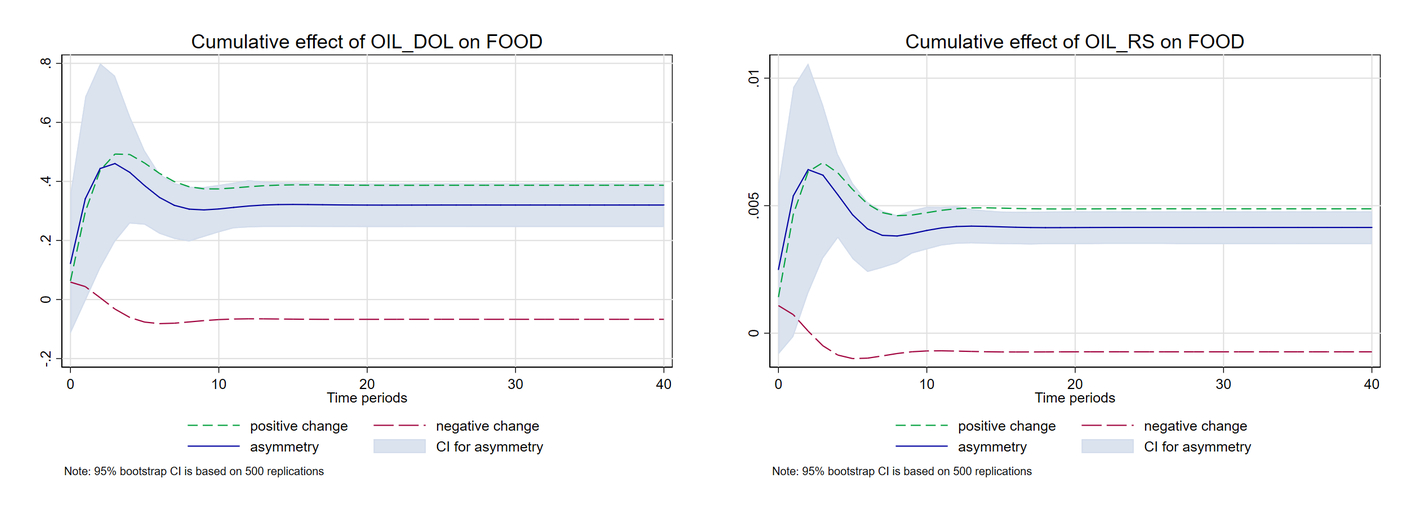
\includegraphics[width=12cm,height=8cm]{Assym_collage.jpg}
	\caption{Dynamic Multipliers of Oil Price Rise and Oil Price Fall }
\end{figure}

Finally, we undertake diagnostic checking for the estimated models. It is observed from the table \ref{tab4} that both models are free from autocorrelation problem upto four lags. The models are also free from ARCH effects upto four lags while the errors in residuals of both the models are normally distributed as indicated by the J-B statistic. Both the models have reasonably high $R^2$ value as well. We also perform the CUSUM and CUSUM squares test to ensure the stability of parameters of both the estimated model. The figures given below indicate that parameters of both the models are stable at 5 percent significance.
\begin{figure}[H]
	\begin{subfigure}{\linewidth}
		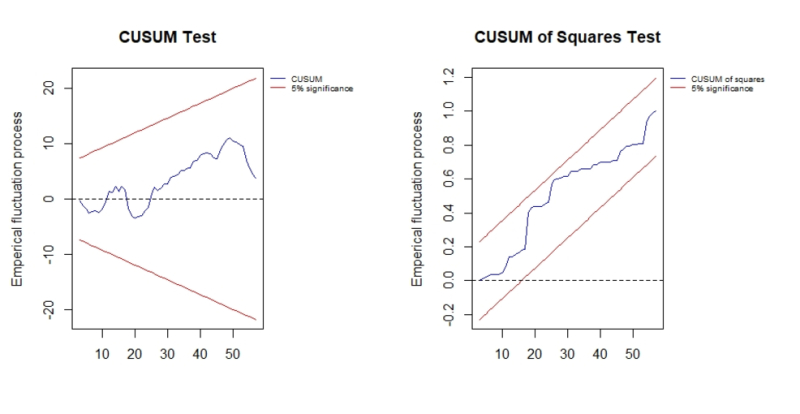
\includegraphics[width=15cm,height=6cm]{cusum_collage}
		\caption{Model 1}
	\end{subfigure}
	\begin{subfigure}{\linewidth}
	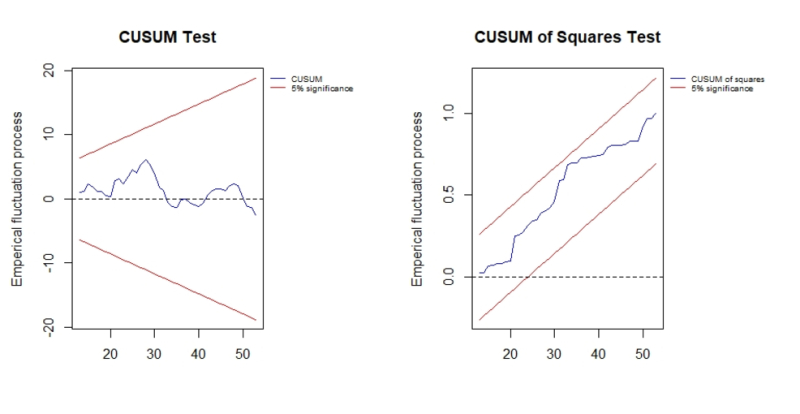
\includegraphics[width=15cm,height=6cm]{cusum2_collage}
	\caption{Model 3}
\end{subfigure}
\caption{CUSUM and CUSUM-Square plots}
\end{figure}

\section{Conclusion}
This paper analyses the potential asymmetry in oil price pass-through to food prices in India. The study uses a NonLinier ARDL framework for capturing the long run and the short run asymmetric relationship between the local food prices and global oil prices. The results of the study indicate the presence of asymmetry in oil price-pass through to food prices in the long run. This oil price price-pass through is higher in case of rupees than compared to dollars which can be due to a depreciation of exchange rate as in 2013 and in the recent past. However, there was no evidence for such asymmetry in the short run both in case of oil price expressed in rupees and in dollars. The presence of asymmetry in the long run has important implications. This also means an increased market power and lesser government intervention to pass the benefits of resuced oil prices to food prices. 
\end{document}
